\begin{quotation}
  {\footnotesize
    \noindent{\emph{``All models are wrong, but some are useful.''\\}
    }
    \begin{flushright}
      George Box
    \end{flushright}
  }
\end{quotation}
\vspace{0.5cm}

\hiddensection{Motivation}
Close range proximity operations between \acrfull{sc}s has been studied and discussed by space agencies and private companies since the early stages of space exploration, dating back to the Apollo program \cite{LangleyApollo}.
Since then we can find a wide range of missions where close-range proximity operations are in, like \acrfull{ff} \cite{2001FormationFliying}  \cite{2009FormationFliying}, \acrfull{oos} \cite{auricchio} \cite{Zimpfer2005} \cite{Tatsch2006} \cite{FloresAbad2014} and \acrfull{adr} \cite{clerc2012astrium} \cite{Bonnal2013}.
Most of those missions were possible thanks to the presence of on-board crew or to the cooperativeness between \acrshort{sc}s.
A target space object is deemed cooperative if it is built to provide information suitable for the estimation of its distance and orientation in space with respect to the chaser \acrshort{sc}. Also, it can be be actively or passively cooperative depending on whether it interacts with a dedicated radio-link with the chaser \acrshort{sc} or not \cite{Opromolla2017}.
As regard to the new generation of space robotics missions such as debris removal and \acrshort{oos}, proximity operations and docking are key-enabling capabilities for either repair, refuel or deorbit end-of-life and nonfunctional \acrshort{sc}s \cite{2016Ventura}.
The main challenge when performing close-range navigation in actual \acrshort{oos} and \acrshort{adr} removal missions however is when the target \acrshort{sc} may be uncooperative.
This implies that the target \acrshort{sc} may not be equipped with an active communication link or identifiable markers such as light-emitting diodes or corner cube reflectors to help with computing the relative position and attitude of the active \acrshort{sc} (chaser) with respect to a uncooperative target space object \cite{2019phdSharma}.
Another important aspect, which comes out when dealing with uncooperative targets, is that debris or operating \acrshort{sc}s to be serviced may have suffered physical damages as well as optical degradation of their surfaces due to the prolonged exposure to the space environment, thus appearing different than expected \cite{Opromolla2017}.
Thus, when operating in close-proximity the attitude and the motion of the target \acrshort{sc} must be estimated in autonomy by exploiting the sensors available on the servicer \acrshort{sc}.
With regards to the technological aspects, \acrfull{eo} sensors have been identified as the best option for relative navigation in the foredescribed scenario \cite{Opromolla2017} \cite{pesciolino}.
Either active Light Detection and Ranging (LIDAR) systems or passive monocular and stereo cameras can be used. The selection of the navigation sensor must consider the resources available on board in terms of mass, electrical and processing power, on one side, the mission scenario and the costs to be sustained for design and development of the satellite system, on the other side \cite{clerc2012astrium} \cite{pesciolino}.
As stated in \cite{Sharma2016} monocular vision navigation has been identified as an enabling technology for present and future \acrshort{ff} and \acrshort{oos} missions (namely PROBA-3 by ESA \cite{Casti2019}, PRISMA by OHB Sweden \cite{2013Damico}).
Monocular navigation on such missions relies on finding an estimate of the initial pose of the space resident object with respect to the camera, based on a minimum number of features from a 3D computer model and a single 2D image \cite{Sharma2016}.
In contrast to other state-of-the-art systems based on \acrfull{lidar} or stero camera sensors, monocular navigation ensures rapid pose determination while offering some advantages such as lower hardware complexity, cost, weight and power consumption, possibility to be simultaneously used for supervised applications and a much larger operational range, not limited by the size of the platform \cite{Sharma2018} \cite{2016Ventura} \cite{pesciolino}.
However, the benefit of lower hardware complexity trades off with increased algorithmic complexity since a monocular sensor cannot provide direct three-dimensional (3D) measurements about the target.
Moreover, monocular sensors can be less robust to adverse illumination conditions typical of the space environment \cite{Volpe2017} (e.g., saturation under direct Sun illumination, or absence of light during eclipse) \cite{pesciolino}.
The increasing challenges of space exploration and moreover the urgent need for debris removal to free slots in orbit and to avoid unwanted collisions is what mainly motivate this work.
The capability of being able to develop and test pose determination algorithm in fact will be a key factor for the overall success of new generation missions. Thus, this work is motivated from the need to implement a low-cost, reliable and extendable solution for simulating spaceborne imagery for \acrfull{cv} alghoritms needs.

\hiddensection{Problem Statement}
The availability of a tool capable of rendering image of the target client \acrshort{sc} is of vital importance for the implementation and testing of any kind of \acrshort{cv} algorithm.
The usage of artificial in images in fact gives a complete control over the scene and more importantly, recently investigated deep learning techniques relies on very huge annotated data-sets of images. The main difficulties when searching for suitable data-sets arises from the difficulty of acquiring thousands of spaceborne images of the desired target \acrshort{sc} with accurately annotated pose labels and with an high enough degree of realism, capable of being representative of real operative conditions. A poorly made data-set in fact can lead to incoherent results due to wrong assumptions, especially when developing techniques which are based on the implementation algorithms relying on Neural Networks. A standard tool capable of generating thousands of images at demands moreover enable the user to systematically evaluate and compare the performance of different algorithms.
So, in this work the possibility of generating an accurate enough dataset by employing Ray-Tracing techniques will be firstly explored. After that, the generated data-set will be employed to implement the \acrfull{svd} monocular pose initialization algorithm.
As stated in \cite{D2014} and \cite{Sharma2018}, the pose initialization problem consist of determining the position of the \acrfull{cg} \gls{t_c} and the orientation of the principal axes \gls{A_TC} of a non-cooperative target \acrshort{sc} (no markers or other specific supportive means) with respect to the camera frame \textbf{C} from a single \acrfull{2d} image, given its \acrfull{3d} geometrical representation (referred as map or model).
If we assume that the \acrshort{3d} model of the target \acrshort{sc} is defined in a body fixed coordinate system \textbf{T}, and it is aligned with the target's principal axes with its origin at the \acrshort{cg}, the orientation is then defined by the \acrfull{dcm} \gls{A_TC}, which represents the trasformation from the coordinate system of \textbf{T} to \textbf{C}.

\begin{figure}[htbp]
  \centering
  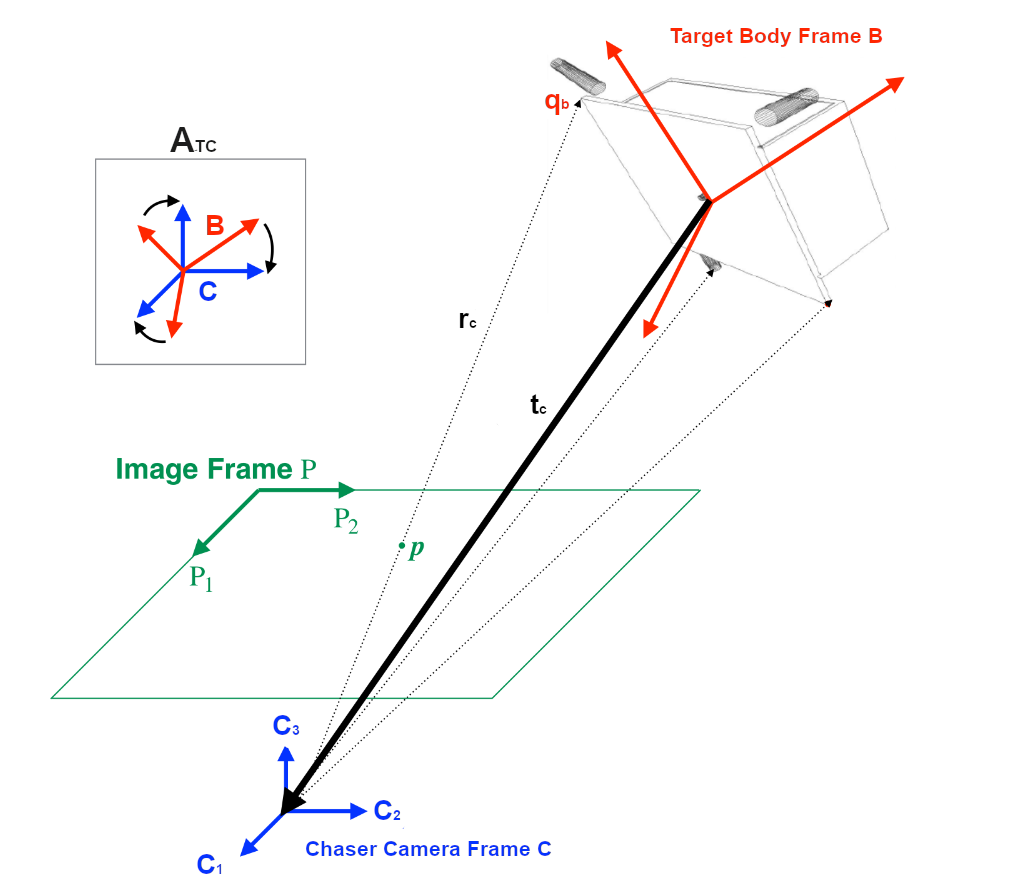
\includegraphics[width=0.82\textwidth]{gfx/poseProblem.eps}
  \caption{Schematic representation of the pose estimation problem using a monocular image \cite{Sharma2018}}
\end{figure}

A generic image point $p$ = $ [u,v]^T $ can be related to the corresponding $\mathbf{q_B}$ point of the \acrshort{3d} model by means of the unknown pose (\gls{t_c} \gls{A_TC}) according to the following \acrshort{2d} - \acrshort{3d} true perspective equations:

\begin{equation}
  \mathbf{r_C} = \left[x_C \quad  y_C \quad z_C\right]^T = \mathbf{A_{TC}} \; \mathbf{q_B} + \mathbf{t_C} \,,
\end{equation}

\begin{equation}
  \mathbf{p} = \left[ \frac{x_C}{z_C} f_x + C_x , \frac{y_C}{z_C} f_y + C_y \right] \,,
\end{equation}

where \gls{fx} and \gls{fy} are the respectively the orizontal and the vertical focal lenght and $[C_x, C_y]$ are the coordinates of the center of the image.\\
As discussed in \cite{D2014}, we can build several considerations on top of those two coupled equations :

\begin{itemize}
  \item the relationship between image points and pose parameter is hightly non linear and the problem of retrieving the \acrshort{3d} points from the \acrshort{2d} image can have infinite solution in under-constrained situations \cite{10.1145/358669.358692};
  \item the correspondence between $\mathbf{q_B}$ and $\mathbf{p}$ is not known \textit{a priori};
  \item the image coordinates need to be corrected for pixel's non-quadratism and lens distortion before using the perspective projection equations.
\end{itemize}

The pose estimation system thus needs the be capable of extracting the client features from the available image (image processing) to obtain measurements, namely  $\mathbf{p}$. The extracted features then needs to be matched to the correspondent elements of a client model (model matching), namely $\mathbf{q_B}$. The unknown pose then has to be estimated based on the available measurements (pose estimation).
The architecture proposed in \cite{Sharma2018} solve the pose estimation problem by coupling the \acrfull{wge} technique with the Sobel edge detection to perform the image processing, uses feature synthesis to reduce the searh space for model matching and combines a \acrshort{pnp} solver with the \acrfull{nr} method for pose estimation.

\hiddensection{Structure of the Thesis}
This thesis work has been divided into four chapters. The first chapter presents to the reader a brief overview on the current state-of-art status for what concerns synthetic images generation for spaceborne applications as well as the autonomous close-proximity relative navigation problem. The second chapter instead is completely focused on the image generation problem, with an in-dept explanation regarding the toolbox which has been developed during this thesis work to allow the end user to produce image data-sets in batch starting from the CAD model of the target \acrshort{sc}. The third chapter is dedicated to the analysis and the implementation of an innovative technique for solving the pose initialization problem when considering non cooperative \acrshort{sc}. The fourth chapter illustrates the results obtained when using the pose initialization algorithm on the images generated with the developed toolbox in order to solve the pose initialization problem. Finally, a conclusion of the work which has been done and a depiction of the possible future developments and research that can be done on both the synthetic images and the algorithm ends the thesis.